% !TEX encoding = UTF-8 Unicode
% $Header: /cvsroot/latex-beamer/latex-beamer/solutions/conference-talks/conference-ornate-20min.en.tex,v 1.6 2004/10/07 20:53:08 tantau Exp $

\documentclass[]{beamer}
\usepackage{icomma}
\usepackage{xltxtra}
\newfontfamily\DejaSans{DejaVu Sans}

% This file is a solution template for:

% - Talk at a conference/colloquium.
% - Talk length is about 20min.
% - Style is ornate.

\mode<presentation>
{
  \usetheme{Warsaw}
  % or ...

  %\setbeamercovered{transparent}
  % or whatever (possibly just delete it)
  
  \setbeamertemplate{navigation symbols}{}
  
  \newcommand*\oldmacro{}%
  \let\oldmacro\insertshorttitle%
  \renewcommand*\insertshorttitle{%
    \oldmacro\hfill%
    \insertframenumber\,/\,\inserttotalframenumber}
}

\usepackage[utf8]{inputenc}
% or whatever

\usepackage{times}
\usepackage{multirow}
\usepackage[T1]{fontenc}
\usepackage{graphicx}
\usepackage{eso-pic}
\usepackage{color}
\usepackage{tikz}
\usepackage{wasysym}
\usepackage{eurosym}
\usepackage{multicol}
\usepackage{booktabs}


% Or whatever. Note that the encoding and the font should match. If T1
% does not look nice, try deleting the line with the fontenc.

\title[]
{Analyzing the data of Mangaki,\\anime \& manga recommender system}

\author[]
{Jill-Jênn Vie}

\institute[]
{
\includegraphics[width=0.42\linewidth]{figures/mangaki.png}}

\date
{Pico Pico Cafe, Kichij\= oji -- May 20, 2017}

\begin{document}

\definecolor{vert}{rgb}{0.07 0.54 0.07}

{
\setbeamertemplate{headline}[default]
\begin{frame}
	\titlepage
\end{frame}
}

\def\R{\mathcal{R}}
\def\N{N}
\newcommand\good{{\color{green!50!black}\DejaSans ☺}}
\newcommand\neutral{{\color{blue}\DejaSans 😐}}
\newcommand\bad{{\color{red}\DejaSans ☹}}

\begin{frame}
  \frametitle{Outline}
  \begin{itemize}
    \item[1.] Who I am
    \item[2.] Mangaki
    \item[3.] How do we make recommendations?
    \item[4.] Demo!
    \item[5.] Further work in adaptive testing
  \end{itemize}
\end{frame}

\begin{frame}
  \frametitle{Hi, I'm JJ}
  \begin{columns}
  \begin{column}{0.7\textwidth}
    \begin{itemize}[<+->]
      \item Researcher in RIKEN AI Project\\
      Between Tokyo and Kyoto University
      \vspace{1.5cm}
      \item Pianist of a French band that performs anime music\\
      \vspace{1.5cm}
      \item Really happy to be in Kichij\= oji tonight!\\
      \uncover<4>{\small (because this is where GTO comes from)}
    \end{itemize}
  \end{column}
  \begin{column}{0.3\textwidth}
  \centering
  
\includegraphics[width=0.4\linewidth]{figures/riken.png}\\[5mm]
  \uncover<2->{
\includegraphics[width=\linewidth]{figures/trioelm.png}\\
  trioelm.com}\\[5mm]
  \uncover<4->{
\includegraphics[width=0.5\linewidth]{figures/gto.png}}
  \end{column}
  \end{columns}
\end{frame}

\begin{frame}
  \frametitle{Let's make the Netflix of manga}
  Because France is the 2\textsuperscript{nd} manga consumer in the world

  \begin{itemize}
    \item[1.] Japan - 500M volumes
    \item[2.] France - 13M volumes \only<2->{(actually, \alert{2\%})}
    \item[3.] US - 9M volumes
  \end{itemize}

  \uncover<3->{\begin{exampleblock}{Mangaki: a non-profit organization founded in 2014}
  \begin{itemize}
  \item 26 members, 10 active: 3 mad developers \& 1 designer
  \item Prize in 2015: Microsoft Ventures (Student Demo Cup)
  \item Prize in 2016: Japanese Cultural Institute in Paris\\[1mm]\hfill\small\em We flew to Tokyo and met Cool Japan Fund!
  \end{itemize}
  \end{exampleblock}}
\end{frame}

\newcommand\discrete[1]{\textcolor{gray}{\hfill {\em \small #1}}}

\begin{frame}
  \frametitle{Mangaki}
    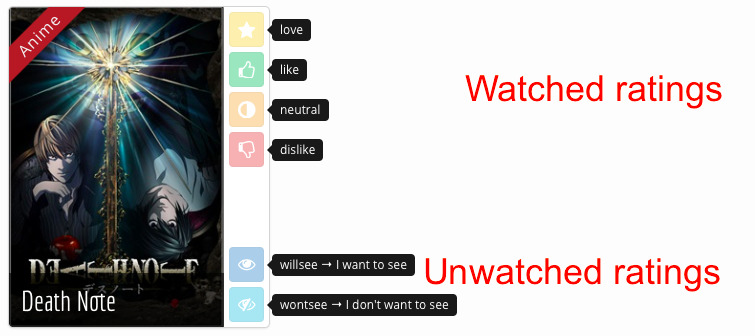
\includegraphics[width=\textwidth]{figures/ratings.jpg}
  \begin{itemize}
  \item 2200 users
  \item 15000 works \discrete{anime / manga / OST}
  \item 325000 ratings \discrete{fav / like / dislike / neutral / willsee / wontsee}
  \item People rate a few works \discrete{Preference Elicitation}
  \item And receive recommendations \discrete{Collaborative Filtering}
  \end{itemize}
\end{frame}

\begin{frame}
	\frametitle{Problem 1: Recommendations}
	\begin{block}{Problem}
		\begin{itemize}
		\item Every user rates some items (1\%)
    \item How to guess the missing ratings?
		\end{itemize}
    \vspace{-2mm}
	\end{block}
  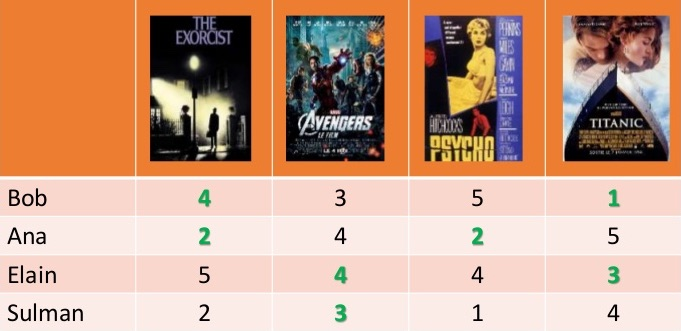
\includegraphics[width=\linewidth]{figures/cf.jpg}
\end{frame}

\begin{frame}[fragile]
  \frametitle{Our anonymized data}
  \begin{verbatim}
user_id,work_id,rating
634,4319,wontsee
1380,6386,willsee
1683,3512,wontsee
1228,6777,like
143,2185,like
816,2805,wontsee
697,6356,wontsee
186,1383,neutral
1666,686,willsee
755,3802,neutral
...
  \end{verbatim}
  \vspace{-7mm}
  (325,000 lines)\bigskip

  Let's do some factor analysis.
\end{frame}

\begin{frame}{Classification problem}

\begin{block}{fit(\(X\), \(y\)) on 325,000 lines of anonymized data}

\centering

\begin{tabular}{ccc} \toprule
\multicolumn{2}{c}{$X$} & $y$\\ \cmidrule{1-2}
\texttt{user\_id} & \texttt{work\_id} & \texttt{rating}\\ \midrule
24 & 823 & like\\
12 & 823 & dislike\\
12 & 25 & favorite\\
\ldots & \ldots & \ldots\\ \bottomrule
\end{tabular}

\pause

\end{block}

\begin{block}{\(\hat{y}\) = predict(\(X\)) the missing entries}

\centering

\begin{tabular}{ccc} \toprule
\multicolumn{2}{c}{$X$} & $\hat{y}$\\ \cmidrule{1-2}
\texttt{user\_id} & \texttt{work\_id} & \texttt{rating}\\ \midrule
24 & 25 & \only<2>{?}\only<3>{\alert{dislike}}\\
12 & 42 & \only<2>{?}\only<3>{\alert{like}}\\ \bottomrule
\end{tabular}

\end{block}

\end{frame}

\begin{frame}{Dimensionality Reduction}

\vspace{-5mm}

\[ R = \left(\begin{array}{c}
\R_1\\
\R_2\\
\vdots\\
\R_n
\end{array}\right) = \raisebox{-1cm}{\begin{tikzpicture}
\draw (0,0) rectangle (2.5,2);
\end{tikzpicture}} =
\raisebox{-1cm}{\begin{tikzpicture}
\draw (0,0) rectangle ++(1,2);
\draw node at (0.5,1) {$C$};
\draw (1.1,1) rectangle ++(2.5,1);
\draw node at (2.35,1.5) {$P$};
\end{tikzpicture}} \]
%\vspace{-2mm}
\[ \text{$R$: 2k users $\times$ 15k works} \iff
\left\{\begin{array}{l}
\text{$C$: 2k users $\times$ \alert{20 profiles}}\\
\text{$P$: \alert{20 profiles} $\times$ 15k works}\\
\end{array}\right. \]
\(\R_\text{Bob}\) is a linear combination of profiles \(P_1\), \(P_2\), etc..

\vspace{5mm}

\pause

\begin{block}{Interpretable profiles \(P_1\), \(P_2\), \(P_3\)}

\begin{tabular}{@{}lccc@{}}
If $P$ & $P_1$ : adventure & $P_2$ : romance & $P_3$ : plot twist\\
And $C_\text{Bob}$ & $0,2$ & $-0,5$ & $0,6$
\end{tabular}

\hfill \(\Rightarrow\) Bob \alert{likes} adventure, \alert{hates} romance, \alert{loves} plot twists.

\end{block}

\pause

Let's keep the 2 first columns of $C$ \& project users on a map.

\end{frame}

\begin{frame}
  \frametitle{user2vec: plotting every user on a map}
  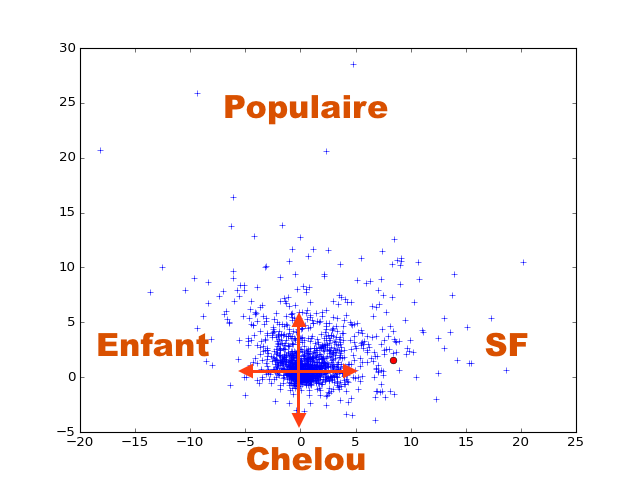
\includegraphics[width=\linewidth]{figures/map.png}
\end{frame}

\begin{frame}
  \frametitle{user2vec: plotting every user on a map}
  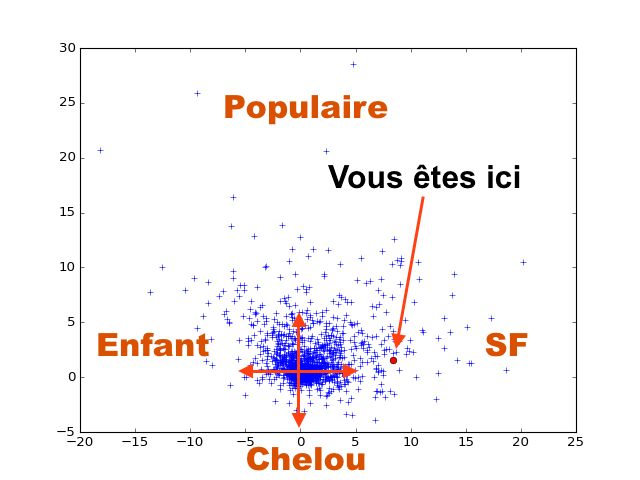
\includegraphics[width=\linewidth]{figures/here.png}
\end{frame}

\begin{frame}
    \frametitle{Mangaki's Explained Profiles}
    \begin{block}{$P_1$ loves Ghibli and cyberpunk, hates teen stories}
    \begin{itemize}
    \item[\good] \emph{Princess Mononoké}, \emph{Spirited Away} (Chihiro)
    \item[\good] \emph{Cowboy Bebop}, space opera similar to \emph{Firefly}
    \item[\good] \emph{Paprika}, which inspired \emph{Inception}
    \item[\bad] \emph{Naruto}, \emph{Bleach}
    \end{itemize}
    \end{block}
    \pause
    \begin{block}{$P_2$ loves really weird works, hates the most popular works}
    \begin{itemize}
    \item[\good] Erotic stories
    \item[\good] Same-family homosexual romances:\\\emph{Kiss x Sis}, \emph{Papa to Kiss in the Dark}
    \item[\bad] \emph{Attack on Titan}, \emph{Death Note}
    \end{itemize}
    \end{block}
\end{frame}

\begin{frame}
  \frametitle{What else can we do with user2vec?}
  \centering \Huge Demo!\vspace{5mm}
  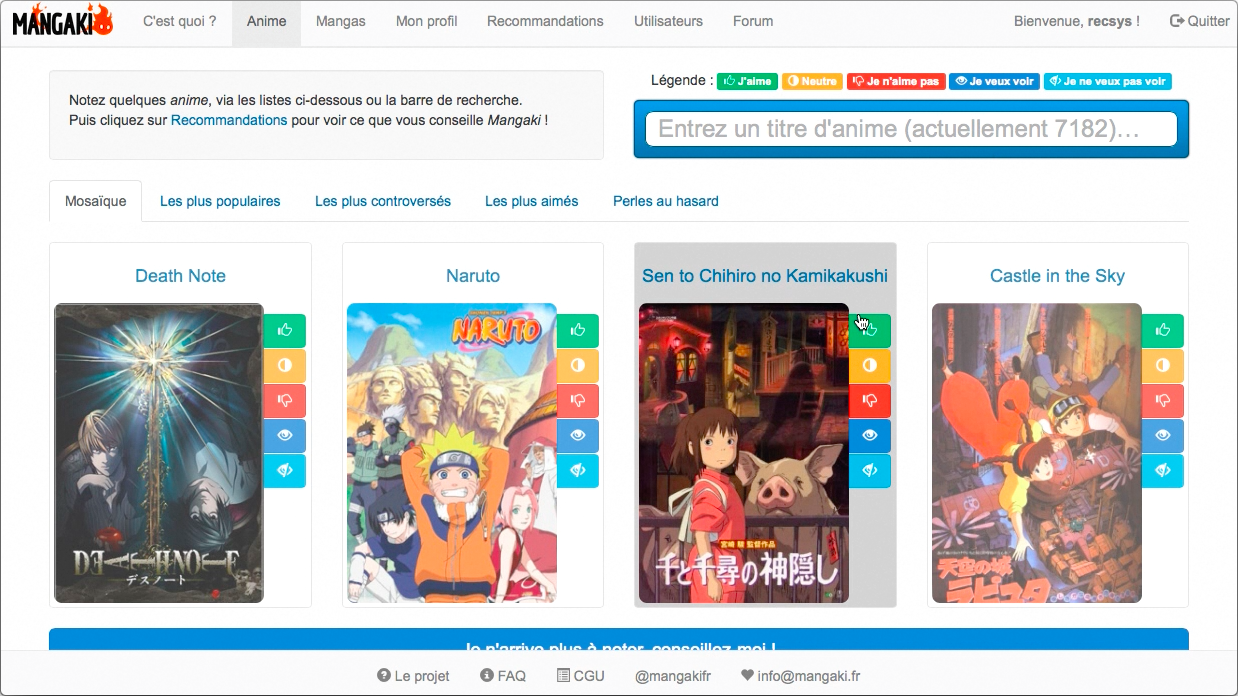
\includegraphics[width=\linewidth]{figures/mangaki-screen.png}\\
\end{frame}

\begin{frame}
  \frametitle{Problem 2: Cold-Start, Preference Elicitation}
  \begin{block}{Problem}
      What questions to ask adaptively to a new user?
  \end{block}
  \centering
  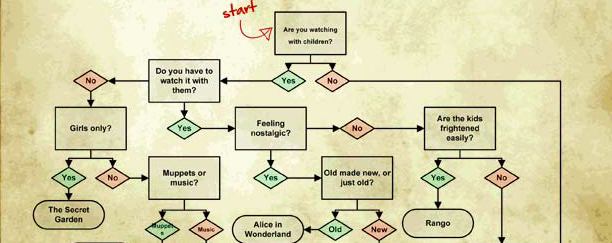
\includegraphics[width=\linewidth]{figures/flowchart.png}\\
  \em What to Watch on Netflix, Silver Oak Casino, 2013
\end{frame}

\begin{frame}
  \frametitle{Actually, Yahoo Labs also is interested in this research}
  \centering
  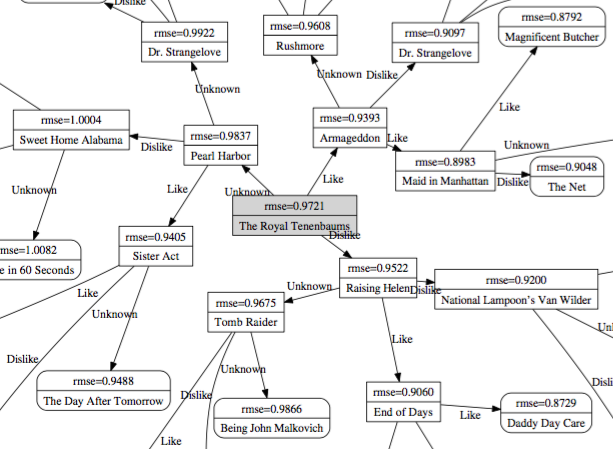
\includegraphics[width=0.9\linewidth]{figures/decisiontree.png}\\
  Good balance between like, dislike and unknown outcomes.
\end{frame}

\begin{frame}
  \frametitle{What questions should be asked?}
  \centering
  points that are \alert{far from each other}\\
  =\\
  \alert{diverse} movies\bigskip

  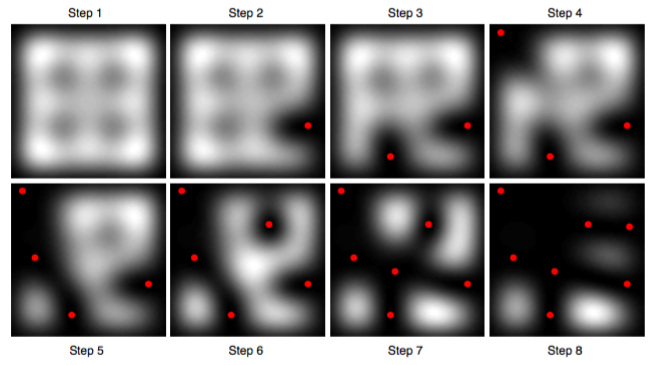
\includegraphics[width=\linewidth]{figures/dpp.png}
\end{frame}

\begin{frame}
  \frametitle{Preference elicitation: sampling a diverse subset}
  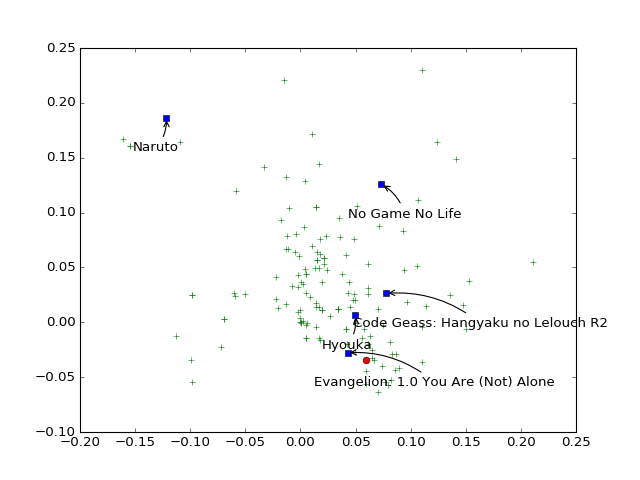
\includegraphics[width=\linewidth]{figures/1.png}
\end{frame}

\begin{frame}
  \frametitle{Summing up \& future work}
  \begin{itemize}
    \item Mangaki is a \alert{non-profit} recommender system\\
    \hfill (discover precious pearls of Japanese animation)\\[5mm]
    \item Mangaki data is a \alert{nice playground for trying algorithms}\\
    \hfill (so far, \texttt{numpy}, \texttt{scikit-learn}, \texttt{tensorflow})\\[5mm]
    \item Organizing a \alert{data challenge} with Kyoto University\\
    \hfill (students will have to work for us for free, {\DejaSans ¥¥¥})\\[5mm]
    \item Use posters as features?\\
    \hfill (\emph{Hey! You seem to like anime that are \textbf{pink}! Booo!!})\\[5mm]
    \item Submitted a proposal for the Anime \& Manga Symposium\\
    \hfill at Anime Expo, Los Angeles, July 1--4, 2017
  \end{itemize}
\end{frame}

\begin{frame}
	\frametitle{Thanks for listening! Feel free to try!}
  \centering
  \LARGE
	
\includegraphics[width=1cm]{figures/twitter.png}\,\,\raisebox{1.5mm}{@MangakiFR (by @jjvie et al.)}
  \vspace{5mm}
  
\includegraphics[width=\linewidth]{figures/mangaki.png}\\
  mangaki.fr \hfill github.com/mangaki
\end{frame}

\end{document}
